\section{Knot colorings}

\subsection{Palettes and diagram colorings}

\hl{An oriented diagram $D$ of knot $K$ has two types of crossings, pictured in} \cref{crossing_type}. A diagram coloring, in essence, is an assignment of values from some mathematical object (i.e. $R$-module) to segments of $D$.

\begin{figure}[h]\centering
  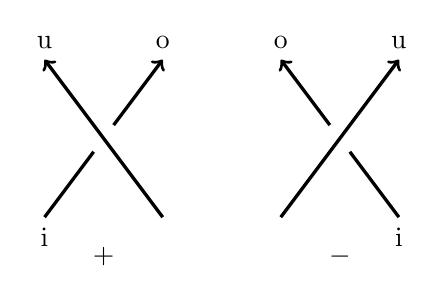
\begin{tikzpicture}
    \draw[very thick, ->] (0,0) node[below] {i} -- (1.5, 2) node[above] {o};
    \fill[white] (0.75, 1) circle (6pt);
    \draw[very thick, ->] (1.5, 0)--(0, 2) node[above] {u};
    \node at (0.75, -0.5) {$+$};

    \draw[very thick, ->] (4.5, 0) node[below] {i} --(3, 2) node[above] {o};
    \fill[white] (3.75, 1) circle (6pt);
    \draw[very thick, ->] (3, 0)--(4.5, 2) node[above] {u};
    \node at (3.75, -0.5) {$-$};
  \end{tikzpicture}
  \caption{Two types of crossing in oriented diagram.\label{crossing_type}}
\end{figure}

\begin{definition}[palette]
  We say that a quadruple {\boldmath$(R, M, \mathcal{C}_\pm)$} is a \buff{palette} if $R$ is a commutative ring with unity, $M$ an $R$-module and $\mathcal{C}_\pm$ are two $R$-modules, corresponding to the two types of crossings (\cref{crossing_type}) such that $\mathcal{C}_\pm\subseteq M^3$.
\end{definition}

We will cumulatively call the two modules $\mathcal{C}_\pm$ the \buff{coloring rule} of palette $(R, M, \mathcal{C}_\pm)$ as they determine whether a coloring is admissible.

\begin{definition}[diagram coloring]
  A \buff{coloring of diagram} $D$ with $s$ segments and $x$ crossings (for knots $s=x$ \cref{ilosc segmentow to ilosc skrzyzowan}) is any element $(m_1,..., m_s)\in M^s$ that assigns elements of $M$ to each arc. 

  We will call a coloring \buff{admissible} if for every crossing $x_j$ of type $\pm$ we have 
  $$\pi_{x_j}(m_1,..., m_s)\in \mathcal{C}_\pm\subseteq\mathcal{C},$$
\hl{where $\pi_{x_j}:M^s\to M^3$ is a projection of module $M^s$ to the $M^3$ factor that corresponds to segments that constitute $x_j$.} 
\end{definition}

Usually, a crossing comprises of exactly three segments. However, as is the case for the first Reidemeister move, a crossing can be comprised of only two segments. Thus, if $x_j$ is such a two-segment crossing, $\im(\pi_{x_j})$ should be isomorphic to $\{(x, y, y)\;:\;x,y\in M\}$.

We can now define two linear homomorphisms
$$\phi_\pm:M^3\to M^3/\mathcal{C}_\pm=N_\pm$$
that take in as arguments the arcs constituting a crossing. Assuming that $M^3/\mathcal{C}_\pm\cong M$ (reasoning behind this assumption will be given in \cref{section 3.2}), we will take 
\begin{align}
  \phi_+(u,i,o)=au+bi+co \label{phi equations1} \\ 
  \phi_-(u,i,o)=\alpha u+\beta i+\gamma o \label{phi equations2}
\end{align}
for $u$, $i$, $o$ understood like in \cref{crossing_type} and with coefficients being homomorphisms $M\to M$.

\begin{lemma}\label{proposition male kernel kolorowania}
  A coloring $(m_1,..., m_s)\in M^s$ is a admissible $\iff$ for each crossing $x_j$ of type $\pm$ 
  $$\phi_\pm(\pi_{x_j}(m_1,...,m_s))=0.$$
\end{lemma}

\begin{proof}
  Stems from the fact that $\mathcal{C}_\pm=\ker\phi_\pm$.
\end{proof}



\subsection{Color checking matrix}
\label{section 3.2}

% We can think of coloring diagrams with a chosen palette $(R, M, \mathcal{C}_\pm)$ as being a {\color{red}functor from a set of diagrams to a set of matrices}.
\hl{Coloring diagrams with a chosen palette $(R, M, \mathcal{C}_\pm)$ is a functor from the category of knot diagrams, whose objects are diagrams and morphisms represent Reidemeister moves, to a category of matrices, with morphisms corresponding to matrix equivalence explained in this section.}

\hl{Moreover, if a palette $P=(R, M, \mathcal{C}_\pm)$ is given alongside a ring homomorphism $f:R\to S$, then an image of this palette $P$ through induced palette homomorphism is $(S, M\otimes_R S, \mathcal{C}_\pm\otimes_R S)$. Similarly, if an $R$-module homomorphism $g:M\to N$ is given, then the image of palette $P$ is $(R, N, g(\mathcal{C}_\pm))$.}

\begin{definition}[color checking matrix]\label{def:color checking matrix}
  Assigning segments of diagram $D$ to coordinates in $M^s$ and crossings to coordinates in $N_\pm^x$ it is possible to define a linear homomorphism $D\phi:M^s\to N_\pm^x$  as
  $$D\phi(m_1,...,m_s)=(\phi_\pm(\pi_{x_1}(m_1,...,m_s)), \phi_\pm(\pi_{x_2}(m_1,...,m_s)),...).$$
  Matrix that is created after choosing a basis for $M^s$ and $N_\pm^x$ will be called a \buff{color checking matrix}.
\end{definition}

\begin{proposition}
  Coloring $(m_1,...,m_s)\in M^s$ is admissible $\iff$ $(m_1,...,m_s)\in\ker D\phi$.
\end{proposition}

\begin{proof}
  We start by saying that 
  $$(m_1,..., m_s)\in\ker D\phi\iff [(\forall\;x_j\text{ crossing})\;\phi_\pm(\pi_{x_j}(m_1,..., m_s))=0].$$
  Which is to say that every coordinate of $D\phi(m_1,..., m_s)$ is zero. Proposition \cref{proposition male kernel kolorowania} says that it is equivalent with $(m_1,..., m_s)$ being an admissible coloring.
\end{proof}

We want to define which color checking matrices are equivalent. We will say that $D\phi$ and $D'\phi$ are equivalent if 
\begin{enumerate}
  \item they differ by a permutation of rows or columns, 
  \item one can be obtained from the other by adding a linear combination of rows or columns to another row or columns 
  \item one can be obtained from the other by adding a new row and a new column with only $0$ save for the term on their intersection, which is a unit.
\end{enumerate}
The first two points mean that two color checking matrices $D\phi, D'\phi:M^s\to N^x$ are equivalent if there exist an isomorphisms $\theta:M^s\to M^s$ and $\psi:N^x\to N^x$ such that
$$
\begin{tikzcd}[column sep=large]
  M^s\arrow[r, "D\phi"]\arrow[d, "\theta" left] & N^x\arrow[d, "\psi" right]\\ 
  M^s\arrow[r, "D'\phi" below] & N^x
\end{tikzcd}
$$
is a commutative diagram. 

In the most basic sense, two diagrams $D$ and $D'$ are isomorphic if there exists an isotopy $h_t:\R^2\to \R^2$ such that $h_0(D)=D$ and $h_1(D)=D'$ and $D'$ has crossings identical to those of $D$.

\begin{lemma}
  Isomorphic diagrams $D\sim D'$ yield equivalent color checking matrices $D\phi\sim D'\phi$.
\end{lemma}

\begin{proof}
  In terms of color checking matrices, an isomorphism of diagrams defined above only relabels segments (permutes columns) and crossings (permutes rows).
\end{proof}

In reality, the isomorphism between diagrams which relates diagrams of the same knot is much more subtle. This relation $R$ is generated by the Reidemeister moves (see \cref{reidemeister-generating}). There is an induced relation on the set of color checking matrices, called $D(R)$, that relates color checking matrices of the same knot. 
\hl{For suitably chosen palettes, an invariant of the equivalent class of matrices of the same knot is known.} 

\begin{definition}[Alexander palette]
One of such palettes is the \buff{Alexander palette} {\boldmath$(R=\Z[\Z], M=\Z[\Z], \mathcal{C}_\pm)$}, where $\mathcal{C}_\pm$ are defined by homomorphisms
$$\phi_+(u,i,o)=(1-t)u+ti-o$$
$$\phi_-(u,i,o)=(1-t^{-1})u+t^{-1}i-o,$$
with $u$, $i$ and $o$ defined in \cref{crossing_type}. 
\end{definition}

For the Alexander palette said invariant is e.g. the determinant of a \hl{$n-1$ minor of the color checking matrix up to multiplication by a unit}. 


The following example illustrates the importance of choosing a suitable palette.

\begin{example}
  Consider a coloring of trefoil knot $3_1$ with two palettes: $P_1=(\Z, \Z, \phi_\pm(u,i,o)=2u-i+o)$ that is not an image of the Alexander palette and $P_2=(\Z, \Z, \phi_\pm(u,i,o)=2u-i-o)$ which in turn is one. The color checking matrix of its diagram with $3$ crossings is
  \begin{center}
    \begin{tikzpicture}
      \begin{knot}[
        consider self intersections, 
        clip width = 20pt, 
        % draft mode=crossings, 
        flip crossing=2
        ] 
        \strand[->, thick] (90:2) to[out=0, in=-60, looseness=2]
        (210:2) to[out=120, in=60, looseness=2]
        (-30:2) to[out=-120, in=180, looseness=2] 
        (90:2);
      \end{knot}

      \node[anchor=west] at (3, 1.8) {
        $P_1(D)=
        \begin{bmatrix}
          2 & -1 & 1\\ 
          -1 & 1 & 2 \\ 
          1 & 2 & -1 
        \end{bmatrix}\mapsto \{1, -3, -5\} 
      $};

    \node[anchor=west] (p2) at (3, -1.2) {
        $P_2(D)=
        \begin{bmatrix}
          2 & -1 & -1\\ 
          -1 & -1 & 2 \\ 
          -1 & 2 & -1 
        \end{bmatrix}\mapsto\{-3\}
      $};
    \end{tikzpicture}
  \end{center}

  while after the first Reidemeister move, the color checking matrix is

  \begin{center}
    \begin{tikzpicture}
      \begin{knot}[
        consider self intersections, 
        clip width = 20pt,
        %ignore endpoint intersections=false,
        % draft mode=crossings,
        % flip crossin=1,
        % flip crossing=2
        ] 
        \strand[<-, thick] (80:3) to[out=-100, in=30] 
        (90:2) to[out=-30, in=-60, looseness=2]
        (210:2) to[out=120, in=60, looseness=2]
        (-30:2) to[out=-120, in=210, looseness=2] 
        (90:2) to[out=150, in=-80] 
        (100:3) to[out=100, in=80, looseness=2] 
        (80:3);
      \end{knot}
      \fill[white] (90:2) circle (10pt);
      \draw[thick] ($(90:2)+({0.3*cos(210)}, {0.3*sin(210)})+(-0.02, -0.07)$) to[out=30, in=-120] ($(90:2) + ({0.3*cos(30}, {0.3*sin(30})+(0, 0.08)$);%(80:3);
      % \draw[->, thin] (90:2) to[out=-30, in=-60, loosenes=2] (210:2);
      
      \node[anchor=west] at (3, 2.5) {$P_1(D)=
          \begin{bmatrix}
            0 & 2 & 1 & -1 \\ 
            0 & -1 & 2 & 1 \\ 
            1 & 0 & -1 & 2\\ 
            1 & 1 & 0 & 0
          \end{bmatrix}\mapsto\{5, 11, 3, ...\}$
        };
      
      \node[anchor=west] at (3, -1) {$P_2(D)=
          \begin{bmatrix}
            0 & 2 & -1 & -1 \\ 
            0 & -1 & 2 & -1 \\ 
            -1 & 0 & -1 & 2\\ 
            -1 & -1 & 0 & 0
          \end{bmatrix}\mapsto\{-3, 3\}$
        };
    \end{tikzpicture}
  \end{center}
\end{example}

In order to ensure that the equivalence classes of color checking matrices under the relation induced by Reidemeister moves on diagrams have a known invariant, rules must be imposed on palettes. A particular set of palettes that will satisfy conditions to be mention are the Alexander palette and all palettes derived from it by either a ring homomorphism or a module homomorphism.

The coloring rule modules $\mathcal{C}_\pm$ are to be isomorphic to $M^2$, with the red arrow being an isomorphism
    $$
    \begin{tikzcd}
      M^2 \arrow[r, hookrightarrow] \arrow[rr, bend right=25, red, "\cong" below] & M^3 \arrow[twoheadrightarrow, r] & \mathcal{C}_\pm.
    \end{tikzcd}
    $$
    We want the red isomorphism to be $(u, i)\mapsto (u, i, \phi_\pm'(u, i))\in\mathcal{C}_\pm$, with segments labeled like in \cref{crossing_type}, meaning that $c$ and $\gamma$ in \eqref{phi equations1} and \eqref{phi equations2} respectively are units. For the sake of convenience, take $c=\gamma=-1$.

    This property of palettes will be called a \buff{propagation rule} as knowing colors of two of the three segments allows one to calculate the color assigned to the remaining segment.

    \begin{lemma}\label{warunki na palete}
  A palette that meets the propagation rule has the following two properties determined by Reidemeister moves.
  \begin{enumerate}
    \item The first Reidemeister move requires that
      $$a=1-b$$
      $$\alpha=1-\beta,$$
      where the variables are coefficients from \eqref{phi equations1} and \eqref{phi equations2}.  
    \item Similarly, the second Reidemeister move requires
      $$\begin{cases}
        a\beta+\alpha=0\\ 
        \beta b=1.
      \end{cases}$$
  \end{enumerate}
\end{lemma}

% {\color{red}from now on we want to work with palettes that satisfy the following conditions: dwuwymiaroowe C i propagation rule, to a = 1-b, b beta = 1 oraz a beta + alpha = 0. in particular, we want to work with the Alexander palette and all palettes derived from it}









\subsection{Reidemeister relation on color checking matrices}

The diagram $D$ has $s$ segments and $x$ crossings and $D\phi:M^s\to N_\pm^x$.

\subsection*{\centering R1}

\begin{center}
  \begin{tikzpicture}
    \draw[->] (0, 0)--(0, 1);
    \draw (0, 1)--(0, 2);
    \draw[dashed] (0, 1) ellipse (0.8 and 1);

    \begin{knot}[
        consider self intersections,
        ignore endpoint intersections=false,
        flip crossing=1,
        clip width=20pt
      ]
      \strand[->] (-3, 0) to[out=90, in=120] (-2.5, 1.3) to[out=-60, in=60] (-2.5, .7) to[out=-120, in=-90] (-3, 2);
    \end{knot}
    \draw[dashed] (-3, 1) ellipse (0.8 and 1);

    \draw[dashed] (3, 1) ellipse (0.8 and 1);
    \begin{knot}[
        consider self intersections,
        ignore endpoint intersections=false,
        clip width=20pt
        %flip crossing=1
      ]
      \strand[->] (3, 0) to[out=90, in=120] (3.5, 1.3) to[out=-60, in=60] (3.5, .7) to[out=-120, in=-90] (3, 2);
    \end{knot}
    \node at (0, -.5) {$D$};
    \node at (3, -.5) {$D_b'$};
    \node at (-3, -.5) {$D_a'$};

    \node at (-3.3, .6) {$x$};
    \node at (-3.3, 1.4) {$y$};

    \node at (2.7, .6) {$x$};
    \node at (2.7, 1.4) {$y$};

    %\node at (.3, .6) {$w$};

    \draw[<->] (-2, 1)--(-1, 1) node[midway, above] {$R1b$};
    \draw[<->] (2, 1)--(1, 1) node[midway, above] {$R1a$};
  \end{tikzpicture}
\end{center}

The first Reidemeister move allows the following two moves on color checking matrices
$$
\begin{matrix}
  D_a' & & D & & D_b'\\ 
  \begin{bmatrix}
    %&X & Y & \hdots\\ 
    b & a+c  & 0 & \hdots\\ 
    x_1 & y_1 & z_1 \\ 
    \vdots & & & \ddots
  \end{bmatrix} 
       & \overset{D(R1a)}{\sim} &
     \begin{bmatrix}
       x_1 + y_1 & z_1 & \hdots\\ 
       \vdots & & \ddots
     \end{bmatrix} 
       & \overset{D(R1b)}{\sim} &
  \begin{bmatrix}
    %&X & Y & \hdots\\ 
    \beta & \alpha+\gamma  & 0 & \hdots\\ 
    x_1 & y_1 & z_1 \\ 
    \vdots & & & \ddots
  \end{bmatrix} 
\end{matrix}
$$
where $(\forall\;i=1,...,x)\;x_i=0\;\lor y_i=0$.

\begin{proof}[{\bfseries Proof of \cref{warunki na palete}.1.}]
% Notice, that if the propagation rule that was outlined at the beginning of this section is to be true, looking closely at the crossing in diagrams above should yield equations
The propagation rule mandates the following equalities
$$0=a+b+c=a+b-1\implies a=1-b$$
$$0=\alpha+\beta+\gamma=\alpha+\beta-1\implies \alpha=1-\beta,$$
as the up and out segments in $D'_a$ and the up and in segments in $D'_b$ must admit coloring with the same element from $M$.
\end{proof}

\subsection*{\centering R2}

\begin{center}
  \begin{tikzpicture}
    \draw[dashed] (0, 0) ellipse (.8 and 1);
    \draw[dashed] (3, 0) ellipse (.8 and 1);

    \begin{knot}[
      % draft mode=crossings, 
      clip width = 4pt,
      flip crossing=1,
      flip crossing=2, 
      % ignore endpoint intersection=false
      ]
      \strand[->] (-75:.8 and 1) to [out=90, in=-90] (0, 0) to[out=90, in=-90] (75:.8 and 1);
      \strand[->] (-105:.8 and 1) to [out=90, in=-90] 
      (.35, 0) to [out=90, in=-90]
      (105:.8 and 1);
    \strand[->] ($(3, 0)+(-75:.8 and 1)$) -- ($(3, 0)+(75:.8 and 1)$);
    \strand[->] ($(3, 0)+(-105:.8 and 1)$) -- ($(3, 0)+(105:.8 and 1)$);
    \end{knot}

    \node at (-.2, -1.5) {$D'$};
    \node at (3, -1.5) {$D$};

    \node at (-.4, 0) {$y$};
    \node at (75:1 and 1.3) {$z$};
    \node at (-75:1 and 1.3) {$x$};
  \end{tikzpicture}
\end{center}

For the second Reidemeister move we will say that $D\phi$ and $D'\phi$ are in relation if they differ by the following matrix move
$$
\begin{matrix}
  D' & & D \\ 
  \begin{bmatrix} 
    b & c & 0 & a & \hdots \\ 
    0 & \beta & \gamma &\alpha \\ 
    x_1 & 0 & z_1 & w_1 \\ 
    \vdots & & & &\ddots
  \end{bmatrix} & \overset{D(R2)}{\sim} &
  \begin{bmatrix} 
       x_1+z_1 & w_1 & \hdots \\ 
       \vdots & & \ddots
     \end{bmatrix}
\end{matrix}
$$
where $(\forall\; i=1,...,x)\;x_i=0\;\lor z_i=0$, in addition to permuting rows and columns and adding linear combination of rows or columns to another row or column.

\begin{proof}[{\bfseries Proof of \cref{warunki na palete}.2.}]
In the case of this Reidemeister move, we would like to be able to color the diagram $D'$ exactly like the diagram $D$ save for the segments contributing to the two additional crossings. This means that segments labeled $z$ and $x$ on the diagram above must admit a coloring with the same element from $M$.

The restrictions stemming from this observation are more easily calculated if homomorphisms $\phi_+$ and $\phi_-$ are made into two matrices, $A_+$ and $A_-$, that take the incoming segments (up and in segments) and return the output segments (out and up segments). This is possible because of the propagation rule.
$$
A_+A_-\begin{bmatrix}u\\i\end{bmatrix}=\begin{bmatrix}
  0 & 1 \\ 
  b & a
  \end{bmatrix}\begin{bmatrix}
  \alpha & \beta \\ 
  1 & 0
\end{bmatrix}
\begin{bmatrix}
  u \\ i 
  \end{bmatrix}=\begin{bmatrix}u\\i\end{bmatrix}
$$
Comparing the terms of the matrix $A_+A_-$ with terms of the identity matrix yields:
$$\begin{cases}
  a\beta+\alpha =0 \\ 
  \beta b=1
\end{cases}$$

\end{proof}

\subsection*{\centering R3}

\begin{center}
  \begin{tikzpicture}
    \begin{knot}[
      % draft mode=crossings, 
      clip width=15pt, 
      flip crossing=1, 
      flip crossing = 2, 
      flip crossing=3, 
      flip crossing=4, 
      flip crossing=6, 
      flip crossing=5
      ]
            \strand[->, thick] (3.8, -5)--(6, -2);
      \strand[->, thick] (4.3, -2)--(6.5, -5);
      \strand[<-, thick] (3.8, -4.2)--(6.5, -4.2);

      \strand[->, thick] (9.5, -5)--(11.7, -2);
      \strand[->, thick] (9, -2)--(11.2, -5);
      \strand[<-, thick] (9, -2.8)--(11.7, -2.8);
    \end{knot}

    \draw[dashed] (3.8, -5)--(6.5, -5)--(6.5, -2)--(3.8, -2)--cycle;
    \draw[dashed] (9, -5) rectangle (11.7, -2);
    
    \node at ( 6.5/2 + 3.8/2, -5.5) {$D$};
    \node at (9/2+11.7/2, -5.5) {$D'$};
  \end{tikzpicture}
\end{center}

% {\large\color{purple}DOKOŃCZYĆ - czy tutaj komutujacy diagram cos da? znaczy w sumie to da, ale to jest jakies dzikie zamienianie wspolrzednych}

The last Reidemeister move does not change the size of matrices but only permutes the terms appearing in columns and rows corresponding to the three crossing that are manipulated in the diagram.
$$
\begin{matrix}
  D' & & D \\ 
  \begin{bmatrix}
    \alpha & \gamma & \beta & 0 & 0 & 0 & \hdots \\ 
    0 & 0 & c & b & 0 & a \\ 
    \beta & 0 & 0 & 0 & \gamma & \alpha \\ 
    u_1 & 0 & v_1 & w_1 & x_4 & y_4 \\ 
    \vdots & & & & & & \ddots
  \end{bmatrix} & \overset{D(R3)}{\sim}
     & 
  \begin{bmatrix}
    0 & 0 & \gamma & \beta & \alpha & 0 & \hdots  \\ 
    \beta & 0 & 0 & 0 & \gamma & \alpha \\ 
    0 & c & b & 0 & 0 & a\\ 
    u_4 & 0 & v_4 & w_4 & x_4 & y_4\\ 
    \vdots & & &  & & \ddots
  \end{bmatrix}
\end{matrix}
$$

Let $D(R)$ be the equivalence relation generated by moves $D(R1a)$, $D(R1b)$, $D(R2)$ and $D(R3)$.

\begin{theorem}\label{theorem macierze sa niezmiennikiem}
  For a diagram $D$ colored with an Alexander palette (or its image) the equivalence class of the color checking matrix $D\phi$ under the equivalence relation $D(R)$ is a knot invariant.
  % The equivalence class of a color checking matrix using the Alexander palette, or its image, of a diagram $D$ under relation $D(R)$ generated by matrix relations $D(R1a)$, $D(R1b)$, $D(R2)$ and $D(R3)$ is a knot invariant. Thus we can define $K\phi:=[D\phi]$.
\end{theorem}

\begin{proof}
  A direct result of the definition of the equivalence relation.
\end{proof}

\Cref{theorem macierze sa niezmiennikiem} justifies defining {\boldmath$K\phi:=[D\phi]$}.


\subsection{Smith normal form}

The ring $R$ of palette $(R, M, \mathcal{C}_\pm)$ is not necessarily a PID ring, e.g. $\Z[\Z]$ ring of the Alexander palette has ideal $(2, t+1)$ which is not principal. However, usually one can find a PID ring $P$ with homomorphism $R\to P$ which creates a new palette $(P, M\otimes_R P, \mathcal{C}_\pm\otimes_R P)$ derived from $(R, M, \mathcal{C}_\pm)$. Matrices over PID rings have many interesting properties, like having a Smith normal form.

\begin{definition}[Smith normal form]
Take $A\in K\phi$ and consider it as an $s\times x$ matrix with terms in a $P$ by the procedure outlined above. Then there exist a $s\times s$ matrix $S$ and $x\times x$ matrix $T$ such that $SAT$ is of form
$$
\begin{bmatrix}
  a_1 & 0 & 0 & \hdots & 0 & \hdots & 0 \\ 
  0 & a_2 & 0\\ 
  0 & 0 & \ddots & & \vdots & & \vdots\\ 
  \vdots & & & a_r\\ 
  0 & & \hdots & & 0 & \hdots & 0 \\ 
  \vdots & & & & \vdots & & \vdots\\ 
  0 & & \hdots & & 0 & \hdots & 0
\end{bmatrix}
$$
where for every $i$ $a_i|a_{i+1}$. Such a matrix $SAT$ is called the \buff{Smith normal form} of matrix $A$.
\end{definition}

The following is an algorithm for computing the Smith normal form of a matrix $A$:

\begin{enumerate}
  \item Let $A=\{a_{i,j}\}_{i,j\leq n}$ be an $n\times n$ matrix. Take the ideal $I=(a_{i,j})_{0<i,j\leq n}$ generated by all the terms of $A$. 
  \item If we are in PID then $I$ has one generator, call it $a$.
  \item We can now use the following row and column operations to put $a$ in the upper left corner of $A$
    \begin{enumerate}
      \item Permuting rows (columns).
      \item Adding a linear combination of rows (columns) to the remaining row (column).
    \end{enumerate}
  \item With $a$ in the upper left corner we can now use the fact that it was the generator of $I$ to strike out the remaining terms on the first column and row, using the operations described in the previous point.
  \item Repeat the same algorithm on the smaller matrix  $\{a_{i,j}\}_{1<i, j\leq n}$.
\end{enumerate}

In \cref{admissible coloring is kernel} we showed that $\overline{x}\in M^n$ is an admissible coloring of a diagram $D$ if and only if $\overline{x}\in\ker D\phi$. The Smith normal form of $D\phi$, when the diagram is colored using the Alexander palette, hints at the structure of matrix kernel - the columns filled with zeros will contributed a factor $M$ to the kernel. 

Similarly, each column of the Smith normal form contains information about the cokernel $\coker(D\phi)$. The columns containing units disappear, the zero columns contribute a free factor while for every other term $a$ which appears on the diagonal, $P/(a)$ is a summand of the cokernel.
This information aligns with the information obtained from the Alexander module, as one can derive the coloring rule of the Alexander palette from the Wirtinger presentation of a diagram.

Consider a crossing
\begin{center}
  \begin{tikzpicture}
    \draw[<-] (0, 0) node[above] {$o$} --(2, 0) node[above] {$i$};
    \fill[white](1, 0) circle (7pt);
    \draw[->] (1, -1) node[right] {$u$}--(1, 1);
  \end{tikzpicture}
\end{center}
and take some $x$ to be the generator that is used to generate a representation for $K_G^{ab}$. Then, the following is a relation in said group:
$$UxCx(Ux)^{-1}=Ix$$
where $U=ux^{-1}$, $I=ix^{-1}$ and $O=ox^{-1}$. 
We can multiply both sides by $x^{-1}$ to obtain
$$x^{-1}UxCU^{-1}=x^{-1}Ix$$
which is change in $\Z[\Z]$ to
$$
tU+C-U=tI\implies 0=(1-t)U+tI-C
$$
The procedure for the other type of crossing is analogous.



% Take $(a)$ to be a prime ideal with its generator $a$ appearing on the diagonal of the Smith normal form of $D\phi$. Then we might consider the matrix over a new ring $P/(a)$, which is still a PID. After this change, the structure of the kernel has changed as now there are additional zero columns where $a$ and all its multiples stood. Meaning that kernel became bigger and more colorings are admissible over $P/(a)$. 


\begin{definition}[reduced normal form of matrix]\label{reduced normal form def}
  Take $A$ to be a matrix with coefficients in principal ideal domain $P$. Take $a_1,...,a_k\in P$ to be all the elements of the Smith normal form of $A$ that are neither zero nor invertible. Consider a new square matrix 
  $$
  \begin{bmatrix}
    a_1 & 0 & 0 & \hdots & 0\\ 
    0 & a_2 & 0 & \hdots & 0 \\ 
    0 & 0 & \ddots & &  \\ 
    \vdots & \vdots & & & \vdots \\ 
    0 & 0 & \hdots & 0 & a_k
  \end{bmatrix}
  $$
  which will be called the \buff{reduced normal form} of matrix $A$.
\end{definition}

Consider the following as a motivation behind \cref{reduced normal form def}.

\begin{example} \label{example reduced normal form}
  \begin{figure}[h]\centering 
    \begin{tikzpicture}
      \coordinate (a1) at (90:6);
      \coordinate (a2) at (0: 2);
      \coordinate (a3) at ($(-90:5.5)+(4, 0)$);
      \coordinate (a4) at (-80:2);
      \coordinate (a5) at (-90:5.5);
      \coordinate (a6) at (-10:5);
      \coordinate (a7) at (30:7);
      \coordinate (a8) at (180:2.5);
      \coordinate (a9) at (-90:3.5);
      \coordinate (a10) at (-10:7);
      \coordinate (a11) at (110:2);

      % \foreach \i in {1,..., 11} \fill (a\i) circle (5pt);

      \begin{knot}[
        consider self intersections, 
        clip width = 20pt,
        % draft mode=crossings, 
        ignore endpoint intersections=false,
        flip crossing=1, 
        flip crossing=3,
        flip crossing=4, 
        flip crossing=5, 
        flip crossing=7, 
        flip crossing=11, 
        flip crossing=12, 
        flip crossing=9
        ]
        \strand[thick] (a1) to[out=-30, in=90] 
        (a2) to[out=-90, in=200] 
        (a3) to[out=20, in=0, looseness=2]
        (a4) to[out=180, in=180, looseness=2] 
        (a5) to[out=0, in=-100] 
        (a6) to[out=80, in=-60] 
        (a7) to[out=120, in=90]
        (a8) to[out=-90, in=180] 
        (a9) to[out=0, in=-90, looseness=2] 
        (a10) to[out=90, in=0]
        (a11) to[out=180, in=150, looseness=1.5]
        (a1);
      \end{knot}
    \end{tikzpicture}
    \caption{A diagram for knot $K11n85$.\label{k11n85 diagram}}
  \end{figure}

  \begin{figure}[h]\centering 
    \begin{tikzpicture}
      \coordinate (a1) at (90:5);
      \coordinate (a2) at (40:3);
      \coordinate (a3) at (-40:3);
      \coordinate (a4) at (-90:5);
      \coordinate (a5) at (-160:3.5);
      \coordinate (a6) at (40:1);
      \coordinate (a7) at (20:6);
      \coordinate (a8) at (80:3);
      \coordinate (a9) at (180+25:1);
      \coordinate (a10) at (130:4);
      \coordinate (a11) at (180:5);
      \coordinate (a12) at (-90:3);
      \coordinate (a13) at (-10:6);
      \coordinate (a14) at (110:2);
      \coordinate (a15) at (110:5);

      % \foreach \i in {1,..., 15} \fill (a\i) circle (5pt);

      \begin{knot}[
        consider self intersections, 
        clip width = 20pt, 
        % draft mode=crossings, 
        flip crossing=1, 
        flip crossing=3, 
        flip crossing=8, 
        flip crossing=4, 
        flip crossing=7, 
        flip crossing=10, 
        flip crossing=9
        ]
        \strand[thick] (a1) to[out=0, in=90] 
        (a2) to[out=-90, in=90] 
        (a3) to[out=-90, in=0] 
        (a4) to[out=180, in=-120]
        (a5) to[out=60, in=150]
        (a6) to[out=-30, in=-90] 
        (a7) to[out=90, in=90, looseness=2] 
        (a8) to[out=-90, in=30]
        (a9) to[out=-150, in=-60]
        (a10) to[out=120, in=90] 
        (a11) to[out=-90, in=180]
        (a12) to[out=0, in=-90] 
        (a13) to[out=90, in=20, looseness=1.5]
        (a14) to[out=-160, in=200, looseness=2]
        (a15) to[out=20, in=180] 
        (a1);
      \end{knot}
    \end{tikzpicture}
    \caption{A diagram for knot $K11n164$.\label{k11n164 diagram}}
  \end{figure}
  Consider the knots $K11n85$ and $K11n164$ pictured in \cref{k11n85 diagram,k11n164 diagram} respectively. They both have the Alexander polynomial equal 
  $$
  \Delta(t)=-t^3+5t^2-10t+13-10t^{-1}+5t^{-2}-t^{-3}.
  $$
  Coloring them with the Alexander palette
  yields two $11\times 11$ matrices whose any $10\times 10$ minor is equal to the Alexander polynomial (up to multiplication by a unit). However, the reduced Smith normal form are distinguishable
  $$D_{11n85}\phi=\begin{bmatrix}
    -t^3+5t^2-10t+13-10t^{-1}+5t^{-2}-t^{-3}
  \end{bmatrix}$$
  $$
  D_{11n164}\phi=\begin{bmatrix}
    1-t+t^2 & 0 \\ 
    0 & -t^{-1}+4-5t+4t^2-t^3
  \end{bmatrix}
  $$
\end{example}
 
\begin{theorem}
  The reduced normal form of color checking matrix does not depend on the choice of diagram $D$. Thus, it is well defined for $K\phi$ and is a knot invariant.
\end{theorem}

\begin{proof}
  \marginnote{nie wiem, czy tutaj aż tak powinno się dokładnie mówić co i jak dodaję?} % TO DO
Take a knot $K$ and its diagram $D$ with $s$ segments and $x$ crossings. We will show that applying any Reidemeister move to this knot will not change the reduced normal form of its color checking matrix.

  \subsection*{\centering R1}

  The first Reidemeister move is split into \textbf{R1a} and \textbf{R1b}. Due to those two cases being analogous, we will focus on the move \textbf{R1a} (the proof of \textbf{R1b} is left as an exercise for the reader).

  Take $D'$ to be diagram $D$ with one arc twisted into a $+$ crossing. In opposition to the assumption in previous section, we will take the arcs and crossings that differ between those two diagrams to be on first positions. Now, the matrices $D\phi$ and $D'\phi$ are as follows
  $$
  D'\phi=
  \begin{bmatrix}
    b & a-1 & 0 & \hdots\\ 
    x_2 & y_2 & \hdots \\ 
    x_3 & y_3 \\ 
    \vdots 
  \end{bmatrix}
  $$
  $$
  D\phi=
  \begin{bmatrix}
    x_2 + y_2 & \hdots \\ 
    x_3 + y_3 \\ 
    \vdots
  \end{bmatrix}
  $$
  Adding the first column of $D'\phi$ to the second column will yield 
  $$
  D'\phi=
  \begin{bmatrix}
    b & 0 & 0 & \hdots\\ 
    x_2 & x_2+y_2 & \hdots \\ 
    x_3 & x_3+y_3 \\ 
    \vdots 
  \end{bmatrix}
  $$
  because $a+b=1$. Now we know that $b$ is a unit, thus we can easily remove the elements of the first column that are not $b$. This results in 
  $$
  D'\phi=
  \begin{bmatrix}
    b & 0 & 0 & \hdots\\ 
    0 & x_2+y_2 & \hdots \\ 
    0 & x_3+y_3 \\ 
    \vdots 
  \end{bmatrix}
  $$
  notice that the lower right portion of this matrix looks exactly like $D\phi$. The only difference is a column containing a singular unit element and thus it will be struck out when computing the reduced normal form. Thus, the reduced normal form of $D'\phi$ is the same as in $D\phi$.
  
  \subsection*{\centering R2}

  Now the diagram $D'$ is a diagram $D$ with one arc poked onto another. Once again we will put those changed arcs at the beggining of the color checking matrix to obtain following matrices:
  $$
  D'\phi=
  \begin{bmatrix}
    \alpha & \beta & -1 & 0 & \hdots \\ 
    a & 0 & b & -1  \\ 
    x_3 & u_3 & 0 & v_3 \\ 
    x_4 & u_4 & 0 & v_4 \\ 
    \vdots & & & & \ddots
  \end{bmatrix}
  $$
  $$
  D\phi= 
  \begin{bmatrix}
    x_3 & u_3 + v_3 & \hdots \\ 
    x_4 & u_4 + v_4 \\ 
    \vdots
  \end{bmatrix}
  $$
  Adding the third column of $D'\phi$ multiplied by $\alpha$ and $\beta$ to first and second column respectively we are able to reduce the first row to only zeros and $-1$. Now, adding this row to the second one creates a column with only $-1$ and zeros. We can put it as the first column:
  $$
  D'\phi=
  \begin{bmatrix}
    -1 & 0 & 0 & 0 & \hdots \\ 
    0 & a +b\alpha & 0 & -1  \\ 
    0 & x_3 & u_3 & v_3 \\ 
    0 & x_4 & u_4 & v_4 \\ 
    \vdots & & & & \ddots
  \end{bmatrix}
  $$
  Notice that $a+b\alpha=0$ and so we can transform this matrix into
  $$
  D'\phi=
  \begin{bmatrix}
    -1 & 0 & 0 & 0 & \hdots \\ 
    0 & -1 & -1 & 0  \\ 
    0 & v_3 +u_3 & v_3+u_3&  x_3 & \\ 
    0 & v_4 +u_4 & v_4+u_4 & x_4 \\ 
    \vdots & & & & \ddots
  \end{bmatrix}
  $$
  and then into 
  $$
  D'\phi=
  \begin{bmatrix}
    -1 & 0 & 0 & 0 & \hdots \\ 
    0 & -1 & 0 & 0  \\ 
    0 & 0 & v_3+u_3&  x_3 & \\ 
    0 & 0 & v_4+u_4 & x_4 \\ 
    \vdots & & & & \ddots
  \end{bmatrix}
  $$
  which obviously has the same reduced normal form as $D\phi$.

  \subsection*{\centering R3}

  $$D\phi=
  \begin{bmatrix}
    \alpha & -1 & \beta & 0 & 0 & 0 \\ 
    0 & 0 & -1 & b & 0 & a \\ 
    \beta & 0 & 0 & 0 & -1 & \alpha \\ 
    u_4 & 0 & v_4 & w_4 & x_4 & y_4
  \end{bmatrix}
  $$
  $$D'\phi=
  \begin{bmatrix}
    0 & 0 & -1 & \beta & \alpha & 0 \\ 
    \beta & 0 & 0 & 0 & -1 & \alpha \\ 
    0 & -1 & b & 0 & 0 & a\\ 
    u_4 & 0 & v_4 & w_4 & x_4 & y_4
  \end{bmatrix}
  $$

  Applying row and column operations on those matrices results in 
  $$
  D\phi=
  \begin{bmatrix}
    -1 & 0 & 0 & 0 & 0 & 0 \\
    0 & -1 & 0 & 0 & 0 & 0 \\ 
    0 & 0 & \beta & 0 & -1 & 0 \\ 
    0 & 0 & u_4+v_4 & w_4+v_4 & x_4-v_4 & y_4+u_4+x_4
  \end{bmatrix}
  $$
  $$
  D'\phi=
  \begin{bmatrix}
    b & 0 & 0 & 0 & 0 & 0 \\
    0 & -\beta & 0 & 0 & 0 & 0 \\ 
    0 & 0 & \beta & 0 & -1 & 0 \\ 
    0 & 0 & u_4+v_4 & w_4+v_4 & x_4-v_4 & y_4+u_4+x_4
  \end{bmatrix}
  $$
  which makes clear that those matrices have the same reduced normal form as $b$ and $\beta$ were taken to be units.

\end{proof}



% \subsection{Diagram colorings}
%
% Let $K$ be a knot and $D$ be its oriented diagram with $s$ segments and $x$ crossings. In such diagrams we can see two different crossing types as seen in \cref{crossing_type}. 
\begin{figure}[h]\centering
  \begin{tikzpicture}
    \draw[->] (0,0) node[below] {i} -- (1.5, 2) node[above] {o};
    \fill[white] (0.75, 1) circle (6pt);
    \draw[->] (1.5, 0)--(0, 2) node[above] {u};
    \node at (0.75, -0.5) {$+$};

    \draw[->] (4.5, 0) node[below] {i} --(3, 2) node[above] {o};
    \fill[white] (3.75, 1) circle (6pt);
    \draw[->] (3, 0)--(4.5, 2) node[above] {u};
    \node at (3.75, -0.5) {$-$};
  \end{tikzpicture}
  \caption{Two types of crossing in oriented diagram.\label{crossing_type}}
\end{figure}

Take a commutative ring with unity $R$ and an $R$-module $M$.

\begin{definition}[coloring rule]
  Take $\mathcal{C}\subseteq M^3\oplus M^3$ to be a module such that there exists two modules $\mathcal{C}_\pm\subseteq M^3$ for which $\mathcal{C}=\mathcal{C}_+\oplus \mathcal{C}_-$. We will call $\mathcal{C}$ a \buff{coloring rule}. The two submodules $\mathcal{C}_\pm$ each correspond to a type of crossing in diagram $D$.
  % There are two submodules $\mathcal{C}_\pm\subseteq \mathcal{C}$, $C=C_++C_-$, each corresponding to a type of crossing in diagram $D$. 
\end{definition}

We can now construct a pair of homomorphisms
% $$\phi:M^3\to M/\mathcal{C}=N$$
$$\phi_\pm:M^3\to M/\mathcal{C}_\pm=N_\pm,$$
cumulatively referred to as $\phi$. We will call $\phi$ and $\mathcal{C}$ \buff{coloring rule} interchangeably.

%Take a commutative ring with unity $R$ and two $R$-modules $M$ and $N$. Take two arbitrary module homomorphisms $\phi_+:M^3\to N$ and $\phi_-:M^3\to N$, one for each type of crossing.

% \begin{definition}[diagram coloring]
%   Let $x_1,..., x_s\in M$ be labels of arcs in diagram $D$. We will say that $(x_1,...,x_s)\in M^s$ is a \buff{coloring} if for every crossing $\pm$ in $D$ consisting of arcs $u$, $i$, $o$ the following relation is satisfied
%   $$\phi_\pm(u,i,o)=0.$$
% \end{definition}

For each crossing $x_j$ in diagram $D$ we can construct a projection 
$$\pi_{x_j}:M^s\twoheadrightarrow M^3$$
which restricts $M^s$ to the three (or two, in which case one coordinate is zero) arcs that constitute $x_j$.

\begin{definition}[diagram coloring]
  A \buff{coloring of diagram} $D$ is any element $(m_1,..., m_s)\in M^s$ that assigns elements of $M$ to each arc. We will call this coloring \buff{admissible} if for every crossing $x_j$ of type $\pm$ we have 
  $$\pi_{x_j}(m_1,..., m_s)\in \mathcal{C}_\pm\subseteq\mathcal{C}.$$
\end{definition}

% It is easy to express admissibility of a coloring in terms of homomorphism $\phi$.

It will be beneficial to express admissibility of a coloring in terms of homomorphisms $\phi$.
\begin{proposition}\label{proposition male kernel kolorowania}
  A coloring $(m_1,..., m_s)\in M^s$ is a admissible $\iff$ for each crossing $x_j$ of type $\pm$ 
  $$\phi_\pm(\pi_{x_j}(m_1,...,m_s))=0.$$
\end{proposition}

\begin{proof}
  Stems from the fact that $\mathcal{C}_\pm=\ker\phi_\pm$.
\end{proof}


%
% \subsection{Color checking matrix}
%
% {\large\color{red}
% tutaj dam definicje color checking matrix z innego pliku
% }
%
% \begin{definition}[color checking matrix]\label{def:color checking matrix}
  After assignings arcs to coordinates in $M^s$ and crossings to coordinates in $N^x$ it is possible to define a linear homomorphism $D\phi:M^s\to N^x$  as
  $$D\phi(m_1,...,m_s)=(\phi_\pm(\pi_{x_1}(m_1,...,m_s)), \phi_\pm(\pi_{x_2}(m_1,...,m_s)),...).$$
  Matrix that is created after choosing a basis for $M^s$ and $N^x$ will be called a \buff{color checking matrix}.
\end{definition}

Taking $\phi_\pm$ to be linear equations of form
$$\phi_+(u,i,o)=au+bi+co$$
$$\phi_-(u,i,o)=\alpha u+\beta i+\gamma o,$$
where $u$, $i$ and $o$ correspond to arcs as seen in \cref{crossing_type} and all the coefficients are linear homomorphisms $M\to N$, we know that all the entries for the color checking matrix will be linear combinations of $a$, $b$, $c$, $\alpha$, $\beta$, $\gamma$. If $M$ has $n$ generators we chose to block the matrix $D\phi$ into $n\times n$ blocks.

\begin{proposition}
  Coloring $(m_1,...,m_s)\in M^s$ is admissible $\iff$ $(m_1,...,m_s)\in\ker D\phi$.
\end{proposition}

\begin{proof}\color{blue}
  $\implies$

  We know that every projection $\pi_{x_j}(m_1,...,m_s)$ is in $\ker\phi_\pm$, depending on the type of $x_j$ crossing. Thus, there is no projection $\pi_{x_j}$ that is not being reduced by $\phi_\pm$.

  $\impliedby$

\end{proof}

{\color{blue}We need to impose restrictions on the coloring rule.} We want $\mathcal{C}$ to be two dimensional (have two generators). That way we have the following diagram
% \begin{center}
% \begin{tikzcd}
%   M^2 & M^3\arrow[l, twoheadrightarrow] \arrow[r, hookleftarrow] & \mathcal{C}\arrow[ll, bend left=20, red, "\sim"]
% \end{tikzcd}
% \end{center}
\begin{center}
\begin{tikzcd}
  M^2 \arrow[r, hookrightarrow] \arrow[rr, bend right=20, red, "\sim" below] & M^3 \arrow[r, twoheadrightarrow] & \mathcal{C}
\end{tikzcd}
\end{center}
We can assume that $M^2$ corresponds to the 'up' and 'in' segments in a crossing (compare \cref{crossing_type}), then we can define $\phi_\pm'$ to take $u$ and $i$ segments and return the out segment so that the labeling agrees with the coloring rule. Now, take the red arrow in the diagram above to be the correspondence
$$(u, i)\mapsto (u, i, \phi_\pm'(u,i)).$$
This demands that both $c$ and $\gamma$ in the definition of $\phi_+$ and $\phi_-$ are invertible. For the sake of simplicity, we will take $c=\gamma=-1$. 

With this assumption for any admissible coloring $(u,i,o)$ of a crossing we have the following relation:
$$\phi_+\;:\;o=au+bi$$
$$\phi_-\;:\;o=\alpha u+\beta i.$$


%it will be beneficial to demand that the red arrow is an isomorphism.
% \begin{enumerate}
%   \item To allow \emph{trivial colorings}, that is colorings in which every arc is assigned the same value it is necessary that
%     $$(\forall\;m\in M)\;\phi_\pm(m,m,m)=0.$$
%   \item To simplify operations of color checking matrices, if
%     $$\phi_+(u, i, o)=au+bi+co$$
%     $$\phi_-(u,i,o)=\alpha u+\beta i+\gamma o,$$
%     then we take $c$ and $\gamma$ to be invertible. For the sake of simplicity, take $c=\gamma=-1$.
%   \item The two variations of orientation of the first Reidemeister move, pictured in \cref{fig: ograniczanie phi reidemeister 1}, put the following constrictions on $a$, $b$ and $\alpha$, $\beta$:
%     $$\begin{cases}
%       a+b=1\\
%       \alpha+\beta=1
%     \end{cases}$$
%   \item Lastly, from the second Reidemeister move, pictured in \cref{fig: ograniczanie phi reidemeister}, one can gather that  
%     $$\begin{cases}
%       a+b\alpha=0\\ 
%       b\beta=1
%     \end{cases}$$
%     meaning that both $b$ and $\beta$ must be units.
% \end{enumerate}
% %
% \begin{figure}[h]\centering
%   \begin{tikzpicture}
%       \begin{knot}[
%         clip width=20pt, 
%         consider self intersections,
%         flip crossing=1
%         ]
%         \strand[thick, ->] (0, 0) to[out=90, in=-90] (0, 1) to[out=90, in=150] (1, 2.5) to[out=-30, in=90] (1.3, 2) to[out=-90, in=30] (1, 1.5) to[out=-150, in=-90] (0, 3) to[out=90, in=-90] (0, 4);
%
%         \strand[thick, ->] (3, 0)--(3, 4);
%
%       \end{knot}
%       \draw[dashed, <->] (1.5, 2)--(2.7, 2);
%
%       \node at (-.5, 2) {$+$};
%       \node at (-1.3, 3.7) {$(a+b)x $};
%       \node at (-.3, -.3) {$x$};
%       \node at (3.3, -.3) {$x$};
%     \begin{scope}[shift={(0, -6)}]
%       \begin{knot}[
%         clip width=20pt, 
%         consider self intersections
%         ]
%         \strand[thick, ->] (0, 0) to[out=90, in=-90] (0, 1) to[out=90, in=150] (1, 2.5) to[out=-30, in=90] (1.3, 2) to[out=-90, in=30] (1, 1.5) to[out=-150, in=-90] (0, 3) to[out=90, in=-90] (0, 4);
%
%         \strand[thick, ->] (3, 0)--(3, 4);
%
%       \end{knot}
%       \draw[dashed, <->] (1.5, 2)--(2.7, 2);
%       \node at (-.5, 2) {$-$};
%
%       \node at (-1.3, 3.7) {$(\alpha+\beta)x $};
%       \node at (-.3, -.3) {$x$};
%       \node at (3.3, -.3) {$x$};
%     \end{scope}
%   \end{tikzpicture}
%   \caption{The two variations of the first Reidemeister move in oriented diagrams. They suggest that $(a+b)=1$ and $(\alpha+\beta)=1$.\label{fig: ograniczanie phi reidemeister 1}}
% \end{figure}
%
% \begin{figure}[h]\centering
%   \begin{tikzpicture}
%     \begin{knot}[
%       clip width=20pt, 
%       flip crossing=1,
%       flip crossing=2
%       ]
%       \strand[thick, ->] (0,-1)--(0, 4);
%       \strand[thick, ->] (-1, -1) to[out=90, in=180+45] (-.8, 0) to[out=45, in=-90] (1, 1.5) to[out=90, in=-45] (-.8, 3) to[out=180-45, in=-90] (-1, 4);
%
%       \strand[thick, ->] (5, -1) -- (5, 4);
%       \strand[thick, ->] (6, -1) -- (6, 4);
%
%     \end{knot}
%     \draw[dashed, <->] (1.5, 1.5)--(4.5, 1.5);
%
%     \node at (-1.3, -.3) {$x$};
%     \node at (.3, -.3) {$y$};
%     \node[anchor=east] at (-.3, 1.5) {$\alpha x+\beta y$};
%     \node[anchor=west] at (.3, 3.7) {$(a+b\alpha) x+b\beta y$};
%
%     \node at (4.7, -.3) {$x$};
%     \node at (6.3, -.3) {$y$};
%
%   \end{tikzpicture}
%   \caption{Second Reidemeister move. It suggests that $(a+b\alpha)=0$ and $b\beta =1$.\label{fig: ograniczanie phi reidemeister}}
% \end{figure}
%
%
% \marginnote{jeszcze przemyśleć tekst}
% It is worth mentioning that examining the second Reidemeister move (\cref{fig: ograniczanie phi reidemeister}) with $\phi_\pm$ changed to $2\times 2$ matrices $A_\pm$, which take arcs entering a crossing as input and output the arcs leaving it, we can see that 
% $$A_+ A_-=\begin{bmatrix}0 & 1\\ b & a\end{bmatrix}\begin{bmatrix}\alpha & \beta \\ 1 & 0\end{bmatrix}=Id.$$
% This means that from homomorphism $\phi_+$ we are able to calculate $\phi_-$ and vice versa.
%
% The color checking matrix is not a knot invariant, despite the restrictions laid on $\phi$. Changing the number of crossings in a diagram will obviously create a different matrix for the same knot. We will thus proceed to define an equivalence relation on the set of all color checking matrices of a knot $K$.

% Let $R$ be a commutative ring, typically $\Z[\Z]$, and take $M,N$ to be two $R$-modules. Consider two module homomorphisms $\phi_+:M^3\to N$ and $\phi_-:M^3\to N$ such that
% $$(\forall\;x\in M)\;\phi_\pm(x,x,x)=0.$$ 
% This homomorphism will be used to determine whether or not a labelling of knot arcs constitutes a coloring or not.
%
% \medskip
%
%
% {\large\color{red}tak naprawdę wystarczy jeden homomorfizm $\phi$, ale nie wiem jeszcze jak to wyjaśnić beż zahaczania o linki lub warkocze}.
% %{\large\color{red}JAK WUTLUMACZYC, ZE NAPRAWDE TO WYSTARCZY JEDNA FUNKCJA, ALE TAK BEDZIE MI LATWIEJ W ZYCIU? BO JAK NARYSUJĘ DIAGRAM Z DWOMA SKRZYŻOWANIAMI JEDNO + A DRUGIE - I POŁĄCZĘ JAK PRZY WARKOCZE -> LINKI TO DOSTAJĘ LINKA Z 2 KOMPONENTAMI :V}
% % It might appear that in the case of oriented diagram two different functions $\phi$ are required. However, considering the following diagram
% % \begin{figure}[h]\centering 
% %   \begin{tikzpicture}
% %     \draw[->] (0,-0.5) to (0, -1) to [out=-90, in=90] (1, -3);
% %     \draw[->] (1, -3) to (1, -3.5) to[out=-90, in=90] (0, -5.5) to (0,-6);
% %
% %     \fill[white] (.5, -2) circle (6pt);
% %     \fill[white] (.5, -4.5) circle (6pt);
% %
% %     \draw[->] (1,-0.5) to (1, -1) to[out=-90, in=90] (0, -3);
% %     \draw[->] (0, -3) to (0, -3.5) to[out=-90, in=90] (1, -5.5) to (1, -6);
% %     \draw (1, -6) to [out=-90, in=-90] (3, -4) to[out=90, in=-90] (3, -2.5) to[out=90, in=90] (1, -.5);
% %
% %     \node at (1, -2) {$-$};
% %     \node at (1, -4.5) {$+$};
% %   \end{tikzpicture}
% %   \caption{Why only one function $\phi$ is required?\label{just_why_phi}}
% % \end{figure}
%
% \medskip
%
%
% The color checking matrix in itself is obviously not a knot invariant. However, we might define an equivalence relation on the set of all matrices $M^m\to N^n$, $m,n\in\N$, such that all the matrices which come from the same knot fall into the same equivalence class.
%



We might also demand that a trivial coloring (every arc is assigned the same element of $M$) is an admissible coloring.

% The color checking matrix is not a knot invariant. Changing the diagram with accordance to the Reidemeister moves might change the dimensions of the matrix. Thus, we need to define an equivalence relation on the set of all color checking matrices.


%
% \subsection{Relation on color checking matrices}
%
% The color checking matrix, defined in \cref{def:color checking matrix}, is not a knot invariant. Its size and structure changes as Reidemeister moves are applied to the diagram. Thus, we need to define which matrices stem from equivalent knot diagrams.

For the time being the diagram $D$ has $s$ segments and $x$ crossings. Although only knots are considered in this paper, it is possible to expand definitions of color checking matrices and relations on them to links.

\subsection*{\centering R1}

\begin{center}
  \begin{tikzpicture}
    \draw[->] (0, 0)--(0, 1);
    \draw (0, 1)--(0, 2);
    \draw[dashed] (0, 1) ellipse (0.8 and 1);

    \begin{knot}[
        consider self intersections,
        ignore endpoint intersections=false,
        flip crossing=1,
        clip width=20pt
      ]
      \strand[->] (-3, 0) to[out=90, in=120] (-2.5, 1.3) to[out=-60, in=60] (-2.5, .7) to[out=-120, in=-90] (-3, 2);
    \end{knot}
    \draw[dashed] (-3, 1) ellipse (0.8 and 1);

    \draw[dashed] (3, 1) ellipse (0.8 and 1);
    \begin{knot}[
        consider self intersections,
        ignore endpoint intersections=false,
        clip width=20pt
        %flip crossing=1
      ]
      \strand[->] (3, 0) to[out=90, in=120] (3.5, 1.3) to[out=-60, in=60] (3.5, .7) to[out=-120, in=-90] (3, 2);
    \end{knot}
    \node at (0, -.5) {$D$};
    \node at (3, -.5) {$D_b'$};
    \node at (-3, -.5) {$D_a'$};

    \node at (-3.3, .6) {$x$};
    \node at (-3.3, 1.4) {$y$};

    \node at (2.7, .6) {$x$};
    \node at (2.7, 1.4) {$y$};

    %\node at (.3, .6) {$w$};

    \draw[<->] (-2, 1)--(-1, 1) node[midway, above] {$R1b$};
    \draw[<->] (2, 1)--(1, 1) node[midway, above] {$R1a$};
  \end{tikzpicture}
\end{center}

Both Reidemeister moves $R1a$ and $R1b$ require the following diagram to commute,
\begin{center}
  \begin{tikzcd}
    M^{s+1}\arrow[r, "D'\phi"]\arrow[d, twoheadrightarrow] & N^{x+1} \arrow[d, twoheadrightarrow] \\ 
    M^{s+1},\; x=y \arrow[d, "f" left] & N^x\oplus (N/\phi_\pm(M^3)) \arrow[d, "g"] \\ 
    M^s \arrow[r, "D\phi" below] & N^x
  \end{tikzcd}
\end{center}
where $\phi_\pm$ changes (for $R1a$ we have $+$ and for $R1b$ $-$). We take $f$ and $g$ to be given by
$$f(m_1,..., m_s, m_{s+1})=(m_1,..., m_s+m_{s+1})$$
$$g(n_1,..., n_x, n_{x+1})=(n_1,..., n_x+n_{x+1}).$$
The homomorphism $f$ ensures that on the rest of diagrams $D'$ arc labeled $x$ in figure above and $y$ add up to the arc visible in the diagram $D$. Meanwhile, $g$ ensures that the additional crossing is treated with the appropriate coloring rule.

In terms of matrices, the above diagram can be translated to
$$
\begin{matrix}
  D_a' & & D & & D_b'\\ 
  \begin{bmatrix}
    %&X & Y & \hdots\\ 
    b & a+c  & 0 & \hdots\\ 
    x_1 & y_1 & z_1 \\ 
    \vdots & & & \ddots
  \end{bmatrix} 
       & \overset{R1a}{\sim} &
     \begin{bmatrix}
       x_1 + y_1 & z_1 & \hdots\\ 
       \vdots & & \ddots
     \end{bmatrix} 
       & \overset{R1b}{\sim} &
  \begin{bmatrix}
    %&X & Y & \hdots\\ 
    \beta & \alpha+\gamma  & 0 & \hdots\\ 
    x_1 & y_1 & z_1 \\ 
    \vdots & & & \ddots
  \end{bmatrix} 
\end{matrix}
$$
where $(\forall\;i=1,...,x)\;x_i=0\;\lor y_i=0$.

Notice, that if the propagation rule that was outlined at the beginning of this section is to be true, one must have
$$0=a+b+c=a+b-1\implies a=1-b$$
$$0=\alpha+\beta+\gamma=\alpha+\beta-1\implies \alpha=1-\beta,$$
as the two segments in both $D'$ must admit coloring with one element from $M$. This puts further restrictions on coloring rules.

\subsection*{\centering R2}

\begin{center}
  \begin{tikzpicture}
    \draw[dashed] (0, 0) ellipse (.8 and 1);
    \draw[dashed] (3, 0) ellipse (.8 and 1);

    \begin{knot}[
      % draft mode=crossings, 
      clip width = 4pt,
      flip crossing=1,
      flip crossing=2, 
      % ignore endpoint intersection=false
      ]
      \strand[->] (-75:.8 and 1) to [out=90, in=-90] (0, 0) to[out=90, in=-90] (75:.8 and 1);
      \strand[->] (-105:.8 and 1) to [out=90, in=-90] 
      (.35, 0) to [out=90, in=-90]
      (105:.8 and 1);
    \strand[->] ($(3, 0)+(-75:.8 and 1)$) -- ($(3, 0)+(75:.8 and 1)$);
    \strand[->] ($(3, 0)+(-105:.8 and 1)$) -- ($(3, 0)+(105:.8 and 1)$);
    \end{knot}

    \node at (-.2, -1.5) {$D'$};
    \node at (3, -1.5) {$D$};

    \node at (-.4, 0) {$y$};
    \node at (75:1 and 1.3) {$z$};
    \node at (-75:1 and 1.3) {$x$};
  \end{tikzpicture}
\end{center}

For the second Reidemeister move we will say that $D\phi$ and $D'\phi$ are in relation if the following diagram commutes:

\begin{center}
  \begin{tikzcd}
    M^{s+2}\arrow[r, "D'\phi"]\arrow[d, twoheadrightarrow] & N^{x+2} \arrow[d, twoheadrightarrow] \\ 
    M^{s+2}, x=z\arrow[d] & N^x\oplus (N/\phi_{\pm}(M^3))\oplus (N/\phi_\mp(M^3))\arrow[d]\\ 
    M^s\arrow[r, "D\phi" ] & N^x
  \end{tikzcd}
\end{center}

In terms of matrices, the following move is admitted:

$$
\begin{matrix}
  D' & D \\ 
  \begin{bmatrix} 
    b & c & 0 & a & \hdots \\ 
    0 & \beta & \gamma &\alpha \\ 
    x_1 & 0 & z_1 & w_1 \\ 
    \vdots & & & &\ddots
  \end{bmatrix} 
     & \begin{bmatrix} 
       x_1+z_1 & w_1 & \hdots \\ 
       \vdots & & \ddots
     \end{bmatrix}
\end{matrix}
$$
where $(\forall\; i=1,...,x)\;x_i=0\;\lor z_i=0$.

Once more, if the propagation property of coloring is to be upheld, then 
$$\begin{cases}
  a\beta+\alpha =0 \\ 
  \beta b=1
\end{cases}$$
meaning that $x$ and $z$ can be colored with one element from $M$.

\subsection*{\centering R3}

\begin{center}
  \begin{tikzpicture}
    \begin{knot}[
      % draft mode=crossings, 
      clip width=15pt, 
      flip crossing=1, 
      flip crossing = 2, 
      flip crossing=3, 
      flip crossing=4, 
      flip crossing=6, 
      flip crossing=5
      ]
            \strand[->, thick] (3.8, -5)--(6, -2);
      \strand[->, thick] (4.3, -2)--(6.5, -5);
      \strand[<-, thick] (3.8, -4.2)--(6.5, -4.2);

      \strand[->, thick] (9.5, -5)--(11.7, -2);
      \strand[->, thick] (9, -2)--(11.2, -5);
      \strand[<-, thick] (9, -2.8)--(11.7, -2.8);
    \end{knot}

    \draw[dashed] (3.8, -5)--(6.5, -5)--(6.5, -2)--(3.8, -2)--cycle;
    \draw[dashed] (9, -5) rectangle (11.7, -2);
    
    \node at ( 6.5/2 + 3.8/2, -5.5) {$D$};
    \node at (9/2+11.7/2, -5.5) {$D'$};
  \end{tikzpicture}
\end{center}

{\large\color{purple}DOKOŃCZYĆ - czy tutaj komutujacy diagram cos da? znaczy w sumie to da, ale to jest jakies dzikie zamienianie wspolrzednych}

In terms of matrices, the following move is admitted: 

$$
\begin{matrix}
  D' & D \\ 
  \begin{bmatrix}
    \alpha & \gamma & \beta & 0 & 0 & 0 & \hdots \\ 
    0 & 0 & c & b & 0 & a \\ 
    \beta & 0 & 0 & 0 & \gamma & \alpha \\ 
    u_1 & 0 & v_1 & w_1 & x_4 & y_4 \\ 
    \vdots & & & & & & \ddots
  \end{bmatrix}
     & 
  \begin{bmatrix}
    0 & 0 & \gamma & \beta & \alpha & 0 & \hdots  \\ 
    \beta & 0 & 0 & 0 & \gamma & \alpha \\ 
    0 & c & b & 0 & 0 & a\\ 
    u_4 & 0 & v_4 & w_4 & x_4 & y_4\\ 
    \vdots & & &  & & \ddots
  \end{bmatrix}
\end{matrix}
$$

\begin{theorem}
  The equivalence class of a color checking matrix of a diagram $D\phi$ under relation generated by matrix relations $R1a$, $R1b$, $R2$ and $R3$ is a knot diagram. Thus we can define $K\phi:=[D\phi]$.
\end{theorem}

\begin{proof}
  A direct result of the definition of the equivalence relation.
\end{proof}

%
% \subsection{Determinant of color checking matrix as a knot invariant}
%
% {\large\color{red}
%   tutaj zostawie restrykcje na color checking matrix tak, zeby wyszedl knot invariant
% }
%
% The reasoning presented in \cref{homological coloring} points at determinant of the coloring matrix being an invariant as was the case for the Alexander matrix. However, at the very moment the color checking matrix is not a knot invariant nor is its determinant. Any module $\mathcal{C}$ and associated with it pair of homomorphisms $\phi$ does not necessarily yield a "nice" coloring. The following example justifies the necessity of imposing restrictions to which a coloring rule must conform in order to be considered in the latter part of this paper.

\begin{example}
  Consider a coloring of trefoil knot $3_1$ with $\Z$ over the ring $\Z$ with $\phi_\pm(u, i, o)=2u-i+o$. The color checking matrix of its diagram with $3$ crossings is
  \begin{center}
    \begin{tikzpicture}
      \begin{knot}[
        consider self intersections, 
        clip width = 20pt, 
        % draft mode=crossings, 
        flip crossing=2
        ] 
        \strand[->, thick] (90:2) to[out=0, in=-60, looseness=2]
        (210:2) to[out=120, in=60, looseness=2]
        (-30:2) to[out=-120, in=180, looseness=2] 
        (90:2);
      \end{knot}

      \node at (6, 0) {
        $\det
        \begin{bmatrix}
          2 & -1 & 1\\ 
          -1 & 1 & 2 \\ 
          1 & 2 & -1 
        \end{bmatrix}=-3
      $};
    \end{tikzpicture}
    \begin{tikzpicture}
      \begin{knot}[
        consider self intersections, 
        clip width = 20pt,
        %ignore endpoint intersections=false,
        % draft mode=crossings,
        % flip crossin=1,
        % flip crossing=2
        ] 
        \strand[<-, thick] (80:3) to[out=-100, in=30] 
        (90:2) to[out=-30, in=-60, looseness=2]
        (210:2) to[out=120, in=60, looseness=2]
        (-30:2) to[out=-120, in=210, looseness=2] 
        (90:2) to[out=150, in=-80] 
        (100:3) to[out=100, in=80, looseness=2] 
        (80:3);
      \end{knot}
      \fill[white] (90:2) circle (10pt);
      \draw[thick] ($(90:2)+({0.3*cos(210)}, {0.3*sin(210)})+(-0.02, -0.07)$) to[out=30, in=-120] ($(90:2) + ({0.3*cos(30}, {0.3*sin(30})+(0, 0.08)$);%(80:3);
      % \draw[->, thin] (90:2) to[out=-30, in=-60, loosenes=2] (210:2);
      \node at (6, 0) {$\det
          \begin{bmatrix}
            0 & 2 & 1 & -1 \\ 
            0 & -1 & 2 & 1 \\ 
            1 & 0 & -1 & 2\\ 
            1 & 1 & 0 & 0
          \end{bmatrix}=-8$
        };
    \end{tikzpicture}
  \end{center}
\end{example}

The most important condition that $\mathcal{C}_\pm$ must meet is to be two dimensional. This will allow for propagation of coloring, meaning that knowing colors of two segments creating a crossing the third one can be calculated from $\phi_\pm$.

The following diagram
% \begin{center}
% \begin{tikzcd}
%   M^2 & M^3\arrow[l, twoheadrightarrow] \arrow[r, hookleftarrow] & \mathcal{C}\arrow[ll, bend left=20, red, "\sim"]
% \end{tikzcd}
% \end{center}
\begin{center}
\begin{tikzcd}
  M^2 \arrow[r, hookrightarrow] \arrow[rr, bend right=20, red, "\sim" below] & M^3 \arrow[r, twoheadrightarrow] & \mathcal{C}
\end{tikzcd}
\end{center}
must commute, with the red arrow being
$$(u, i)\mapsto (u, i, \phi_\pm'(u, i))$$
where $\phi_\pm'$ calculates the "out" segment in admissible coloring of each crossing (compare \cref{crossing_type}). Using (\ref{phi equations1}) and (\ref{phi equations2}) we can take $c$ and $\gamma$ to be any invertible elements, i.e. $c=\gamma=-1$, to have 
$$\phi_+'(u,i)=au+bi$$
$$\phi_-'(u,i)=\alpha u+\beta i$$

Notice that now a diagram with all but one segments colored can be easily colored in its entirety, using $\phi_\pm'$ on the crossing where the remaining segment starts.

 
%
% \subsection{Reduced Smith normal form}
%
% The ring $R$ over which we consider modules $M$ is not necessary a principal ideal domain. However, there are plenty of PID rings and more often than not, one can find at least one PID $P$ with a homomorphism $R\to P$ that allows to consider $M$ as a $P$-module by tensoring it with $P$:
$$M_P=M\otimes_R P.$$
We will use this idea to define a new type of equivalence relation on any color checking matrices.

\begin{definition}[Smith normal form]
Take $A\in K\phi$ and consider it as an $n\times n$ matrix with terms in a $P$ by the procedure outlined above. Then there exist a $n\times n$ matrix $S$ and $n\times n$ matrix $T$ such that $SAT$ is of form
$$
\begin{bmatrix}
  a_1 & 0 & 0 & \hdots & 0 & \hdots & 0 \\ 
  0 & a_2 & 0\\ 
  0 & 0 & \ddots & & \vdots & & \vdots\\ 
  \vdots & & & a_r\\ 
  0 & & \hdots & & 0 & \hdots & 0 \\ 
  \vdots & & & & \vdots & & \vdots\\ 
  0 & & \hdots & & 0 & \hdots & 0
\end{bmatrix}
$$
where for every $i$ $a_i|a_{i+1}$. Such a matrix $SAT$ is called the \buff{Smith normal form} of matrix $A$.
\end{definition}

As was mentioned in the first section, $\overline{x}\in M^n$ is a coloring of a diagram $D$ if and only if $D\phi(\overline{x})=0$, that is $\overline{x}\in\ker D\phi$. The Smith normal form hints at the structure of matrix kernel - the columns filled with zeros will contributed a "free" factor $M$ to the kernel. 

Take $(a)$ to be a prime ideal with its generator $a$ appearing in the Smith normal form of $D\phi$. Then we might consider the matrix over a new ring $P/(a)$, which is still a PID. After this change, the structure of the kernel has changed as now there are additional zero columns where $a$ and all its multiples stood. Meaning that kernel became bigger and more colorings are admissible over $P/(a)$.

\begin{definition}[reduced normal form of matrix]\label{reduced normal form def}
  Take $A$ to be a matrix with coefficients in principal ideal domain $P$. Take $a_1,...,a_k\in P$ to be all the elements of the Smith normal form of $A$ that are neither zero nor invertible. Consider a new square matrix 
  $$
  \begin{bmatrix}
    a_1 & 0 & 0 & \hdots & 0\\ 
    0 & a_2 & 0 & \hdots & 0 \\ 
    0 & 0 & \ddots & &  \\ 
    \vdots & \vdots & & & \vdots \\ 
    0 & 0 & \hdots & 0 & a_k
  \end{bmatrix}
  $$
  which will be called the \buff{reduced normal form} of matrix $A$.
\end{definition}

%{\color{purple}
  When working with knots we usually take $R=\Z[t, t^{-1}]$ and $M=\Z[t, t^{-1}]$. This is not a PID ring but there are multitudes of PID rings into which $R$ can be mapped. The following algorithm can be used to calculate the Smith normal form of a color checking matrix over a PID ring.
  %, however we might want to try and calculate the Smith normal form of the color checking matrix without changing to PID.

  \begin{enumerate}
    \item Let $A=\{a_{i,j}\}_{i,j\leq n}$ be an $n\times n$ matrix. Take the ideal $I=(a_{i,j})$ generated by all the terms of $A$. 
    \item If we are in PID then $I$ has one generator, call it $a$.
    \item We can now use the following row and column operations to put $a$ in the upper left corner of $A$
      \begin{enumerate}
        \item Permuting rows (columns).
        \item Adding a linear combination of rows (columns) to the remaining row (column).
      \end{enumerate}
    \item With $a$ in the upper left corner we can now use the fact that it was the generator of $I$ to strike out the remaining terms on the first column and row, using the operations described in the previous point.
    \item Repeat the same algorithm on the smaller matrix  $\{a_{i,j}\}_{1<i, j\leq n}$.
  \end{enumerate}
%}

The following example justifies the utility of the reduced normal form of color checking matrices in distinguishing knots.

\begin{example} \label{example reduced normal form}
  \begin{figure}[h]\centering 
    \begin{tikzpicture}
      \coordinate (a1) at (90:6);
      \coordinate (a2) at (0: 2);
      \coordinate (a3) at ($(-90:5.5)+(4, 0)$);
      \coordinate (a4) at (-80:2);
      \coordinate (a5) at (-90:5.5);
      \coordinate (a6) at (-10:5);
      \coordinate (a7) at (30:7);
      \coordinate (a8) at (180:2.5);
      \coordinate (a9) at (-90:3.5);
      \coordinate (a10) at (-10:7);
      \coordinate (a11) at (110:2);

      % \foreach \i in {1,..., 11} \fill (a\i) circle (5pt);

      \begin{knot}[
        consider self intersections, 
        clip width = 20pt,
        % draft mode=crossings, 
        ignore endpoint intersections=false,
        flip crossing=1, 
        flip crossing=3,
        flip crossing=4, 
        flip crossing=5, 
        flip crossing=7, 
        flip crossing=11, 
        flip crossing=12, 
        flip crossing=9
        ]
        \strand[thick] (a1) to[out=-30, in=90] 
        (a2) to[out=-90, in=200] 
        (a3) to[out=20, in=0, looseness=2]
        (a4) to[out=180, in=180, looseness=2] 
        (a5) to[out=0, in=-100] 
        (a6) to[out=80, in=-60] 
        (a7) to[out=120, in=90]
        (a8) to[out=-90, in=180] 
        (a9) to[out=0, in=-90, looseness=2] 
        (a10) to[out=90, in=0]
        (a11) to[out=180, in=150, looseness=1.5]
        (a1);
      \end{knot}
    \end{tikzpicture}
    \caption{A diagram for knot $K11n85$.\label{k11n85 diagram}}
  \end{figure}

  \begin{figure}[h]\centering 
    \begin{tikzpicture}
      \coordinate (a1) at (90:5);
      \coordinate (a2) at (40:3);
      \coordinate (a3) at (-40:3);
      \coordinate (a4) at (-90:5);
      \coordinate (a5) at (-160:3.5);
      \coordinate (a6) at (40:1);
      \coordinate (a7) at (20:6);
      \coordinate (a8) at (80:3);
      \coordinate (a9) at (180+25:1);
      \coordinate (a10) at (130:4);
      \coordinate (a11) at (180:5);
      \coordinate (a12) at (-90:3);
      \coordinate (a13) at (-10:6);
      \coordinate (a14) at (110:2);
      \coordinate (a15) at (110:5);

      % \foreach \i in {1,..., 15} \fill (a\i) circle (5pt);

      \begin{knot}[
        consider self intersections, 
        clip width = 20pt, 
        % draft mode=crossings, 
        flip crossing=1, 
        flip crossing=3, 
        flip crossing=8, 
        flip crossing=4, 
        flip crossing=7, 
        flip crossing=10, 
        flip crossing=9
        ]
        \strand[thick] (a1) to[out=0, in=90] 
        (a2) to[out=-90, in=90] 
        (a3) to[out=-90, in=0] 
        (a4) to[out=180, in=-120]
        (a5) to[out=60, in=150]
        (a6) to[out=-30, in=-90] 
        (a7) to[out=90, in=90, looseness=2] 
        (a8) to[out=-90, in=30]
        (a9) to[out=-150, in=-60]
        (a10) to[out=120, in=90] 
        (a11) to[out=-90, in=180]
        (a12) to[out=0, in=-90] 
        (a13) to[out=90, in=20, looseness=1.5]
        (a14) to[out=-160, in=200, looseness=2]
        (a15) to[out=20, in=180] 
        (a1);
      \end{knot}
    \end{tikzpicture}
    \caption{A diagram for knot $K11n164$.\label{k11n164 diagram}}
  \end{figure}
  Consider the knots $K11n85$ and $K11n164$ pictured in \cref{k11n85 diagram,k11n164 diagram}. They both have the Alexander polynomial equal 
  $$
  \Delta(t)=-t^3+5t^2-10t+13-10t^{-1}+5t^{-2}-t^{-3}.
  $$
  Coloring them over ring $\Z[\Z]$ with module $M=\Z[\Z]$ and coloring rules
  $$
  \phi_+(u, i, o)=(1-t)u+tb-o
  $$
  $$
  \phi_-(u,i,o)=(1-t^{-1})y+t^{-1}b-o
  $$
  yields two $11\times 11$ matrices whose any $10\times 10$ minor is equal to the Alexander polynomial (up to multiplication by a unit). However, the reduced Smith normal form are 
  $$D_{11n85}\phi=\begin{bmatrix}
    -t^3+5t^2-10t+13-10t^{-1}+5t^{-2}-t^{-3}
  \end{bmatrix}$$
  $$
  D_{11n164}\phi=\begin{bmatrix}
    1-t+t^2 & 0 \\ 
    0 & -t^{-1}+4-5t+4t^2-t^3
  \end{bmatrix}
  $$
\end{example}

Having witnessed the utility of the reduced normal form of a coloring matrix we proceed to show that it is in fact a knot invariant.

\begin{theorem}
  The reduced normal form of color checking matrix does not depend on the choice of diagram $D$. Thus, it is well defined for $K\phi$ and is a knot invariant.
\end{theorem}

\begin{proof}
  \marginnote{nie wiem, czy tutaj aż tak powinno się dokładnie mówić co i jak dodaję?} % TO DO
Take a knot $K$ and its diagram $D$ with $s$ segments and $x$ crossings. We will show that applying any Reidemeister move to this knot will not change the reduced normal form of its color checking matrix.

  \subsection*{\centering R1}

  The first Reidemeister move is split into \textbf{R1a} and \textbf{R1b}. Due to those two cases being analogous, we will focus on the move \textbf{R1a} (the proof of \textbf{R1b} is left as an exercise for the reader).

  Take $D'$ to be diagram $D$ with one arc twisted into a $+$ crossing. In opposition to the assumption in previous section, we will take the arcs and crossings that differ between those two diagrams to be on first positions. Now, the matrices $D\phi$ and $D'\phi$ are as follows
  $$
  D'\phi=
  \begin{bmatrix}
    b & a-1 & 0 & \hdots\\ 
    x_2 & y_2 & \hdots \\ 
    x_3 & y_3 \\ 
    \vdots 
  \end{bmatrix}
  $$
  $$
  D\phi=
  \begin{bmatrix}
    x_2 + y_2 & \hdots \\ 
    x_3 + y_3 \\ 
    \vdots
  \end{bmatrix}
  $$
  Adding the first column of $D'\phi$ to the second column will yield 
  $$
  D'\phi=
  \begin{bmatrix}
    b & 0 & 0 & \hdots\\ 
    x_2 & x_2+y_2 & \hdots \\ 
    x_3 & x_3+y_3 \\ 
    \vdots 
  \end{bmatrix}
  $$
  because $a+b=1$. Now we know that $b$ is a unit, thus we can easily remove the elements of the first column that are not $b$. This results in 
  $$
  D'\phi=
  \begin{bmatrix}
    b & 0 & 0 & \hdots\\ 
    0 & x_2+y_2 & \hdots \\ 
    0 & x_3+y_3 \\ 
    \vdots 
  \end{bmatrix}
  $$
  notice that the lower right portion of this matrix looks exactly like $D\phi$. The only difference is a column containing a singular unit element and thus it will be struck out when computing the reduced normal form. Thus, the reduced normal form of $D'\phi$ is the same as in $D\phi$.
  
  \subsection*{\centering R2}

  Now the diagram $D'$ is a diagram $D$ with one arc poked onto another. Once again we will put those changed arcs at the beggining of the color checking matrix to obtain following matrices:
  $$
  D'\phi=
  \begin{bmatrix}
    \alpha & \beta & -1 & 0 & \hdots \\ 
    a & 0 & b & -1  \\ 
    x_3 & u_3 & 0 & v_3 \\ 
    x_4 & u_4 & 0 & v_4 \\ 
    \vdots & & & & \ddots
  \end{bmatrix}
  $$
  $$
  D\phi= 
  \begin{bmatrix}
    x_3 & u_3 + v_3 & \hdots \\ 
    x_4 & u_4 + v_4 \\ 
    \vdots
  \end{bmatrix}
  $$
  Adding the third column of $D'\phi$ multiplied by $\alpha$ and $\beta$ to first and second column respectively we are able to reduce the first row to only zeros and $-1$. Now, adding this row to the second one creates a column with only $-1$ and zeros. We can put it as the first column:
  $$
  D'\phi=
  \begin{bmatrix}
    -1 & 0 & 0 & 0 & \hdots \\ 
    0 & a +b\alpha & 0 & -1  \\ 
    0 & x_3 & u_3 & v_3 \\ 
    0 & x_4 & u_4 & v_4 \\ 
    \vdots & & & & \ddots
  \end{bmatrix}
  $$
  Notice that $a+b\alpha=0$ and so we can transform this matrix into
  $$
  D'\phi=
  \begin{bmatrix}
    -1 & 0 & 0 & 0 & \hdots \\ 
    0 & -1 & -1 & 0  \\ 
    0 & v_3 +u_3 & v_3+u_3&  x_3 & \\ 
    0 & v_4 +u_4 & v_4+u_4 & x_4 \\ 
    \vdots & & & & \ddots
  \end{bmatrix}
  $$
  and then into 
  $$
  D'\phi=
  \begin{bmatrix}
    -1 & 0 & 0 & 0 & \hdots \\ 
    0 & -1 & 0 & 0  \\ 
    0 & 0 & v_3+u_3&  x_3 & \\ 
    0 & 0 & v_4+u_4 & x_4 \\ 
    \vdots & & & & \ddots
  \end{bmatrix}
  $$
  which obviously has the same reduced normal form as $D\phi$.

  \subsection*{\centering R3}

  $$D\phi=
  \begin{bmatrix}
    \alpha & -1 & \beta & 0 & 0 & 0 \\ 
    0 & 0 & -1 & b & 0 & a \\ 
    \beta & 0 & 0 & 0 & -1 & \alpha \\ 
    u_4 & 0 & v_4 & w_4 & x_4 & y_4
  \end{bmatrix}
  $$
  $$D'\phi=
  \begin{bmatrix}
    0 & 0 & -1 & \beta & \alpha & 0 \\ 
    \beta & 0 & 0 & 0 & -1 & \alpha \\ 
    0 & -1 & b & 0 & 0 & a\\ 
    u_4 & 0 & v_4 & w_4 & x_4 & y_4
  \end{bmatrix}
  $$

  Applying row and column operations on those matrices results in 
  $$
  D\phi=
  \begin{bmatrix}
    -1 & 0 & 0 & 0 & 0 & 0 \\
    0 & -1 & 0 & 0 & 0 & 0 \\ 
    0 & 0 & \beta & 0 & -1 & 0 \\ 
    0 & 0 & u_4+v_4 & w_4+v_4 & x_4-v_4 & y_4+u_4+x_4
  \end{bmatrix}
  $$
  $$
  D'\phi=
  \begin{bmatrix}
    b & 0 & 0 & 0 & 0 & 0 \\
    0 & -\beta & 0 & 0 & 0 & 0 \\ 
    0 & 0 & \beta & 0 & -1 & 0 \\ 
    0 & 0 & u_4+v_4 & w_4+v_4 & x_4-v_4 & y_4+u_4+x_4
  \end{bmatrix}
  $$
  which makes clear that those matrices have the same reduced normal form as $b$ and $\beta$ were taken to be units.

\end{proof}

 
